\documentclass[11pt,a4paper]{article}

\usepackage[a4paper,margin=1in]{geometry}
\usepackage{amsmath}
\usepackage{amssymb}
\usepackage{array}
\usepackage{booktabs}
\usepackage{enumitem}
\usepackage{tabularx}
\usepackage[T1]{fontenc}
\usepackage{lmodern}
\usepackage{tikz}
\usepackage{xcolor}

\definecolor{packblue}{RGB}{26,68,114}
\definecolor{packgrey}{RGB}{85,85,85}

\setlength{\parindent}{0pt}
\setlength{\parskip}{0.45em}
\setlist[enumerate,1]{label=(\alph*), leftmargin=1.1cm, itemsep=0.55em, topsep=0.4em}

\begin{document}

\begin{center}
{\Large\bfseries\color{packblue} Week 10 Revision Selected Questions}\\[0.4em]
{\large Worked Solutions}\\[0.3em]
{\color{packgrey} Based on \texttt{Sem 2 Week 10 - Revision.pdf}}
\end{center}

\vspace{0.8em}
\hrule
\vspace{1em}

\textbf{1. GreenGrid Energy}

Let $x_A,\ldots,x_F \in \{0,1\}$ where $x_i=1$ if project $i$ is selected.

\begin{enumerate}
\item A suitable binary model is
\[
\max Z = 14x_A+17x_B+11x_C+20x_D+9x_E+15x_F
\]
subject to
\[
6x_A+8x_B+5x_C+9x_D+4x_E+7x_F \le 21
\]
\[
x_D \le x_B
\]
\[
x_A+x_F \le 1
\]
\[
x_C+x_E \ge 1
\]
\[
x_i \in \{0,1\} \quad \text{for all projects } i.
\]

\item The optimal solution is
\[
x_B=x_D=x_E=1,\qquad x_A=x_C=x_F=0.
\]
Total cost:
\[
8+9+4=21
\]
Total benefit:
\[
17+20+9=46.
\]
So the best project set is $\{B,D,E\}$ with maximum total annual benefit score $46$.

\item Binary variables are required because each project is indivisible.
It is meaningful to choose or reject a project, but not to choose, for example, 0.4 of project $D$.

\item Add the constraint
\[
x_A+x_B+x_C+x_D+x_E+x_F=4.
\]
Under the budget and logic rules, there is no feasible solution selecting exactly four projects.
So the revised model is infeasible.

\item One realistic extension would be a multi-period capital budgeting model with separate yearly budgets and project timing decisions.
This would need extra data on when costs are incurred, when benefits begin, and any project sequencing dependencies.
\end{enumerate}

\newpage

\textbf{2. Hock-Brooke Automobiles}

\fbox{\parbox{0.95\linewidth}{\small\textbf{Corrected 15 Oct 2026 (erratum C1).} The earlier version used a spreadsheet in which the \emph{Delivered} and \emph{Demand} tables were swapped (and the demand values shifted by one), and it charged overflow on the closing stock. This version uses the data as set, charges space on the stock held during the week (opening stock + Monday delivery), and reports expected costs over a 52-week horizon. The notebook \texttt{Hock-Brooke - warehouse simulation.ipynb} reproduces every figure.}}

New cars arrive on Monday and are collected on Friday or Saturday, so during the week the dealer must hold the leftover stock \emph{plus} the delivery. For a capacity $c$, the weekly cost is $10c + 20\max(0,\ \text{stock}-c)$; sales are $\min(\text{stock},\text{demand})$ and unsold cars carry over.

\begin{enumerate}
\item For capacity 9, an illustrative 12-week simulation (random draws for deliveries and demand) is:

\begin{center}
\begin{tabular}{ccccccccc}
\toprule
Week & Opening & Delivered & Stock held & Demand & Sales & Closing & Overflow & Cost \\
\midrule
1 & 0 & 9 & 9 & 6 & 6 & 3 & 0 & 90 \\
2 & 3 & 8 & 11 & 7 & 7 & 4 & 2 & 130 \\
3 & 4 & 9 & 13 & 10 & 10 & 3 & 4 & 170 \\
4 & 3 & 10 & 13 & 7 & 7 & 6 & 4 & 170 \\
5 & 6 & 9 & 15 & 6 & 6 & 9 & 6 & 210 \\
6 & 9 & 8 & 17 & 8 & 8 & 9 & 8 & 250 \\
7 & 9 & 7 & 16 & 7 & 7 & 9 & 7 & 230 \\
8 & 9 & 9 & 18 & 8 & 8 & 10 & 9 & 270 \\
9 & 10 & 8 & 18 & 9 & 9 & 9 & 9 & 270 \\
10 & 9 & 10 & 19 & 6 & 6 & 13 & 10 & 290 \\
11 & 13 & 10 & 23 & 10 & 10 & 13 & 14 & 370 \\
12 & 13 & 9 & 22 & 7 & 7 & 15 & 13 & 350 \\
\bottomrule
\end{tabular}
\end{center}

This run costs $2800$ over 12 weeks, i.e.\ $2800/12 \approx 233.33$ per week. Overflow grows because the mean delivery ($8.80$ cars) exceeds the mean demand ($8.65$): unsold stock tends to build up by about $0.15$ cars a week, so there is no stable long-run average and the answer depends on the horizon. Over one year (52 weeks, starting empty) the \emph{expected} average weekly cost for capacity 9 is
\[
\approx 243.78 \text{ per week}
\]
(exact Markov-chain calculation; 2,000 simulated years give $\approx 242.5$).

\item Expected average weekly cost over 52 weeks, starting with an empty warehouse:

\begin{center}
\begin{tabular}{lc}
\toprule
Capacity & Average Weekly Cost \\
\midrule
6 & 272.57 \\
7 & 262.57 \\
8 & 252.84 \\
9 & 243.78 \\
10 & 236.48 \\
11 & 230.81 \\
12 & 226.54 \\
13 & 223.64 \\
14 & 222.01 \\
15 & 221.56 \textbf{(lowest)} \\
16 & 222.22 \\
17 & 223.89 \\
18 & 226.49 \\
\bottomrule
\end{tabular}
\end{center}

So capacity 9 is not the best choice. Over a year the lowest expected cost is at about \textbf{15 spaces} ($\approx 221.56$ per week), with 14 and 16 within $\pounds 1$. Over a shorter 12-week horizon the best is 11 spaces ($\approx 137.85$ per week). Because stock keeps building up, the dealer should also review the order quantity, not only the warehouse size.

Note: other correctly executed simulations will give different short-run tables; the expected values above do not depend on the random numbers.
\end{enumerate}

\newpage

\textbf{3. University Library Help Desk}

\begin{enumerate}
\item Main components:

Entities: students.

Resource: advisers.

Events: arrival, service start, service completion.

Stochastic inputs: interarrival times and service times.

Performance measures: number served, average wait, maximum wait and the percentage waiting less than 8 minutes.

\item One valid baseline run gives:

\begin{center}
\begin{tabular}{lc}
\toprule
Measure & Result \\
\midrule
Students served & 41 \\
Average wait & 1.17 minutes \\
Maximum wait & 10.32 minutes \\
\% waiting less than 8 minutes & 95.12\% \\
\bottomrule
\end{tabular}
\end{center}

\item Peak-period results:

\begin{center}
\begin{tabular}{lcccc}
\toprule
Advisers & Served & Avg wait & Max wait & \% below 8 min \\
\midrule
2 & 70 & 1.88 & 12.99 & 95.71\% \\
3 & 73 & 0.32 & 3.22 & 100.00\% \\
4 & 70 & 0.08 & 2.23 & 100.00\% \\
\bottomrule
\end{tabular}
\end{center}

The target is 97\% waiting less than 8 minutes.
The minimum staffing level that meets the target is therefore 3 advisers.

\item A \texttt{PriorityResource} can be used instead of an ordinary \texttt{Resource}.
Each arrival is labelled priority or standard, for example with probability 0.10 of being priority.
Priority users would request service with a smaller priority number, such as \texttt{priority=0}, while standard users might request with \texttt{priority=1}.
This would generally reduce waits for priority users and increase waits for standard users.

\item A single run is not enough because simulation output is affected by random variation.
Replications with different seeds give more stable estimates and allow the calculation of confidence intervals.
If the system were modelled as an ongoing operation rather than a fixed 360-minute session, a warm-up period could also be used to reduce start-up bias.
\end{enumerate}

\newpage

\textbf{4. F.B. Knight Deliveries}

Because the costs are stated per 10 items, it is convenient to model the variables in tens of items.
Then warehouse supplies are 10, 10 and 10, while shop demands are 7, 8 and 15.

\begin{enumerate}
\item Let
\[
x_{ij}=\text{number of tens of items shipped from warehouse }i\text{ to shop }j
\]
for
\[
i \in \{A,B,C\}, \qquad j \in \{X,Y,Z\}.
\]

The direct transportation network is:

\begin{center}
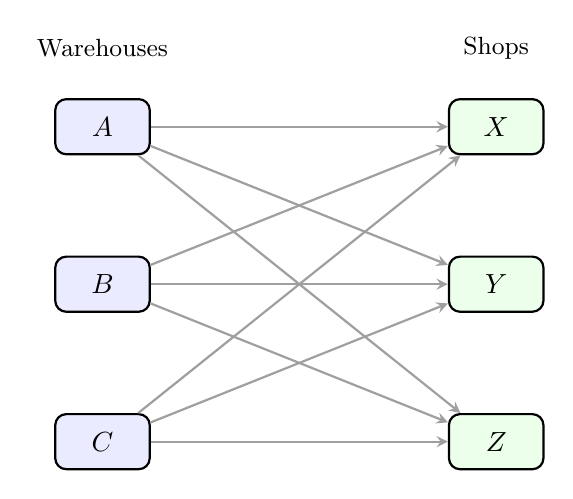
\begin{tikzpicture}[>=stealth, line width=0.8pt]
\node[draw, rounded corners, minimum width=1.2cm, minimum height=0.7cm, fill=blue!8] (A) at (0,2) {$A$};
\node[draw, rounded corners, minimum width=1.2cm, minimum height=0.7cm, fill=blue!8] (B) at (0,0) {$B$};
\node[draw, rounded corners, minimum width=1.2cm, minimum height=0.7cm, fill=blue!8] (C) at (0,-2) {$C$};
\node[draw, rounded corners, minimum width=1.2cm, minimum height=0.7cm, fill=green!8] (X) at (5,2) {$X$};
\node[draw, rounded corners, minimum width=1.2cm, minimum height=0.7cm, fill=green!8] (Y) at (5,0) {$Y$};
\node[draw, rounded corners, minimum width=1.2cm, minimum height=0.7cm, fill=green!8] (Z) at (5,-2) {$Z$};
\foreach \i in {A,B,C} {
  \foreach \j in {X,Y,Z} {
    \draw[->, gray!75] (\i) -- (\j);
  }
}
\node at (0,3) {\small Warehouses};
\node at (5,3) {\small Shops};
\end{tikzpicture}
\end{center}

The direct-shipping transportation model is
\[
\min Z =
8x_{AX}+7x_{AY}+5x_{AZ}
+12x_{BX}+3x_{BY}+9x_{BZ}
+10x_{CX}+11x_{CY}+7x_{CZ}
\]
subject to warehouse supply constraints
\[
x_{AX}+x_{AY}+x_{AZ}=10
\]
\[
x_{BX}+x_{BY}+x_{BZ}=10
\]
\[
x_{CX}+x_{CY}+x_{CZ}=10
\]
shop demand constraints
\[
x_{AX}+x_{BX}+x_{CX}=7
\]
\[
x_{AY}+x_{BY}+x_{CY}=8
\]
\[
x_{AZ}+x_{BZ}+x_{CZ}=15
\]
and non-negativity:
\[
x_{ij}\ge 0.
\]

One optimal direct-shipping plan is:

\begin{center}
\begin{tabular}{lcc}
\toprule
Route & Quantity (tens of items) & Cost per 10 items \\
\midrule
$A \to Z$ & 10 & 5 \\
$B \to X$ & 2 & 12 \\
$B \to Y$ & 8 & 3 \\
$C \to X$ & 5 & 10 \\
$C \to Z$ & 5 & 7 \\
\bottomrule
\end{tabular}
\end{center}

Total cost:
\[
10(5)+2(12)+8(3)+5(10)+5(7)=183.
\]

\item With the restrictions
\[
x_{BY}=0
\]
and
\[
x_{AY}\ge 0.5
\]
the same arc-variable model is modified by adding
\[
x_{BY}=0
\]
and
\[
x_{AY}\ge 0.5.
\]

In tens-of-items units, one optimal revised plan is:

\begin{center}
\begin{tabular}{lc}
\toprule
Route & Quantity (tens of items) \\
\midrule
$A \to Y$ & 8 \\
$A \to Z$ & 2 \\
$B \to X$ & 7 \\
$B \to Z$ & 3 \\
$C \to Z$ & 10 \\
\bottomrule
\end{tabular}
\end{center}

Revised total cost:
\[
8(7)+2(5)+7(12)+3(9)+10(7)=247.
\]
So the extra restrictions increase the cost from 183 to 247.

\item If direct shipping is not allowed and the intermediary locations are used, define arc variables
\[
y_{ik}=\text{flow from warehouse }i\text{ to intermediary }k
\]
for
\[
i \in \{A,B,C\}, \qquad k \in \{D_1,D_2\}
\]
and
\[
z_{kj}=\text{flow from intermediary }k\text{ to shop }j
\]
for
\[
k \in \{D_1,D_2\}, \qquad j \in \{X,Y,Z\}.
\]

The transhipment network is:

\begin{center}
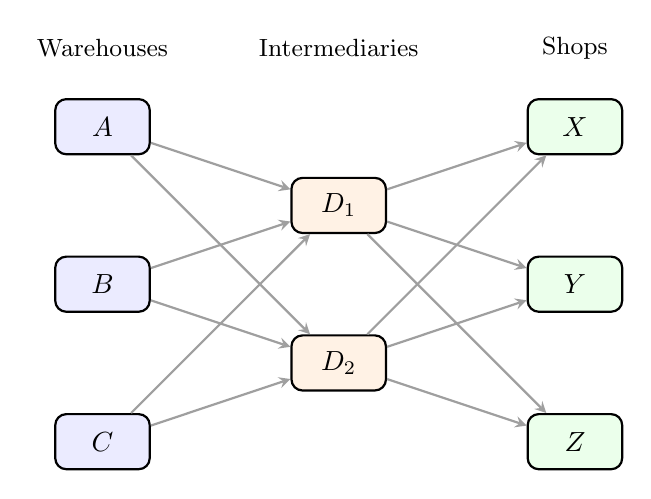
\begin{tikzpicture}[>=stealth, line width=0.8pt]
\node[draw, rounded corners, minimum width=1.2cm, minimum height=0.7cm, fill=blue!8] (A) at (0,2) {$A$};
\node[draw, rounded corners, minimum width=1.2cm, minimum height=0.7cm, fill=blue!8] (B) at (0,0) {$B$};
\node[draw, rounded corners, minimum width=1.2cm, minimum height=0.7cm, fill=blue!8] (C) at (0,-2) {$C$};
\node[draw, rounded corners, minimum width=1.2cm, minimum height=0.7cm, fill=orange!10] (D1) at (3,1) {$D_1$};
\node[draw, rounded corners, minimum width=1.2cm, minimum height=0.7cm, fill=orange!10] (D2) at (3,-1) {$D_2$};
\node[draw, rounded corners, minimum width=1.2cm, minimum height=0.7cm, fill=green!8] (X) at (6,2) {$X$};
\node[draw, rounded corners, minimum width=1.2cm, minimum height=0.7cm, fill=green!8] (Y) at (6,0) {$Y$};
\node[draw, rounded corners, minimum width=1.2cm, minimum height=0.7cm, fill=green!8] (Z) at (6,-2) {$Z$};
\foreach \i in {A,B,C} {
  \foreach \k in {D1,D2} {
    \draw[->, gray!75] (\i) -- (\k);
  }
}
\foreach \k in {D1,D2} {
  \foreach \j in {X,Y,Z} {
    \draw[->, gray!75] (\k) -- (\j);
  }
}
\node at (0,3) {\small Warehouses};
\node at (3,3) {\small Intermediaries};
\node at (6,3) {\small Shops};
\end{tikzpicture}
\end{center}

The transhipment model is
\[
\min Z =
4y_{AD_1}+5y_{AD_2}
+3y_{BD_1}+2y_{BD_2}
+6y_{CD_1}+4y_{CD_2}
+4z_{D_1X}+5z_{D_1Y}+2z_{D_1Z}
+2z_{D_2X}+4z_{D_2Y}+4z_{D_2Z}
\]
subject to supply constraints at the warehouses
\[
y_{AD_1}+y_{AD_2}=10
\]
\[
y_{BD_1}+y_{BD_2}=10
\]
\[
y_{CD_1}+y_{CD_2}=10
\]
demand constraints at the shops
\[
z_{D_1X}+z_{D_2X}=7
\]
\[
z_{D_1Y}+z_{D_2Y}=8
\]
\[
z_{D_1Z}+z_{D_2Z}=15
\]
and flow-balance constraints at the intermediary nodes
\[
y_{AD_1}+y_{BD_1}+y_{CD_1}=z_{D_1X}+z_{D_1Y}+z_{D_1Z}
\]
\[
y_{AD_2}+y_{BD_2}+y_{CD_2}=z_{D_2X}+z_{D_2Y}+z_{D_2Z}.
\]

All arc flows satisfy
\[
y_{ik}\ge 0, \qquad z_{kj}\ge 0.
\]

If only one intermediary is used, then the variables on the unused node are omitted from the model.
The three possibilities are:

\begin{center}
\begin{tabular}{lc}
\toprule
Intermediary choice & Total cost \\
\midrule
$D_1$ only & 228 \\
$D_2$ only & 216 \\
Both $D_1$ and $D_2$ & 181 \\
\bottomrule
\end{tabular}
\end{center}

So both intermediary locations should be used.

One optimal transhipment plan is:

\begin{center}
\begin{tabular}{lc}
\toprule
Route & Quantity (tens of items) \\
\midrule
$A \to D_1$ & 10 \\
$B \to D_1$ & 5 \\
$B \to D_2$ & 5 \\
$C \to D_2$ & 10 \\
$D_1 \to Z$ & 15 \\
$D_2 \to X$ & 7 \\
$D_2 \to Y$ & 8 \\
\bottomrule
\end{tabular}
\end{center}

Total cost:
\[
10(4)+5(3)+5(2)+10(4)+15(2)+7(2)+8(4)=181.
\]
This is slightly cheaper than the best direct-shipping plan.
\end{enumerate}

\newpage

\textbf{5. Forecasting at N\&F}

\begin{enumerate}
\item The quarterly data show a clear upward trend over time.
Using centred 4-quarter moving averages, the smoothed values where available are:

\begin{center}
\begin{tabular}{cc}
\toprule
Period & Centred 4-quarter moving average \\
\midrule
3 & 1020.250 \\
4 & 1030.500 \\
5 & 1040.750 \\
6 & 1050.625 \\
7 & 1060.500 \\
8 & 1070.375 \\
9 & 1080.375 \\
10 & 1090.625 \\
11 & 1100.875 \\
12 & 1111.125 \\
13 & 1121.250 \\
14 & 1131.000 \\
\bottomrule
\end{tabular}
\end{center}

\item Estimated seasonal variations:

Additive seasonal values:
\[
\text{Spring}=12.48,\quad
\text{Summer}=15.85,\quad
\text{Autumn}=-18.27,\quad
\text{Winter}=-10.06.
\]

Multiplicative seasonal indices:
\[
\text{Spring}=1.0117,\quad
\text{Summer}=1.0147,\quad
\text{Autumn}=0.9829,\quad
\text{Winter}=0.9907.
\]

\item A linear trend fitted to the centred moving averages is approximately
\[
\hat{T}_t = 990.12 + 10.07t.
\]

Forecasts for next year are therefore:

\begin{center}
\begin{tabular}{lccc}
\toprule
Period & Season & Additive Forecast & Multiplicative Forecast \\
\midrule
17 & Spring & 1173.74 & 1174.83 \\
18 & Summer & 1187.18 & 1188.53 \\
19 & Autumn & 1163.12 & 1161.18 \\
20 & Winter & 1181.40 & 1180.42 \\
\bottomrule
\end{tabular}
\end{center}

\item Both models give very similar forecasts.
However, the additive model is slightly easier to justify because the seasonal effects appear roughly constant in size over time, rather than increasing proportionally with the level of the series.
So an additive model would be a reasonable recommendation here, although either model would give very similar practical forecasts.
\end{enumerate}

\vfill

\begin{center}
\textit{End of Solutions}
\end{center}

\end{document}
